\documentclass[a4paper,twoside]{article}
\usepackage[T1]{fontenc}
\usepackage[bahasa]{babel}
\usepackage{graphicx}
\usepackage{graphics}
\usepackage{subcaption}
\usepackage{float}
\usepackage[]{hyperref}
\usepackage[cm]{fullpage}
\usepackage{xspace}
%\usepackage{multicol} % for multiple columns
\pagestyle{myheadings}
\usepackage{etoolbox}
\usepackage{setspace} 
\usepackage{lipsum} 
\setlength{\headsep}{30pt}
\usepackage[inner=2cm,outer=2.5cm,top=2.5cm,bottom=2cm]{geometry} %margin
% \pagestyle{empty}

\makeatletter
\renewcommand{\@maketitle} {\begin{center} {\LARGE \textbf{ \textsc{\@title}} \par} \bigskip {\large \textbf{\textsc{\@author}} }\end{center} }
\renewcommand{\thispagestyle}[1]{}
\markright{\textbf{\textsc{AIF184001/AIF184002 \textemdash Rencana Kerja Skripsi \textemdash Sem. Genap 2021/2022}}}

\newcommand{\HRule}{\rule{\linewidth}{0.4mm}}
\renewcommand{\baselinestretch}{1}
\setlength{\parindent}{0 pt}
\setlength{\parskip}{6 pt}

\graphicspath{{./Gambar/}}% folder tempat gambar 
%untuk url dan link
\hypersetup{unicode=true,colorlinks=true,linkcolor=blue,citecolor=green,filecolor=magenta, urlcolor=cyan}

\onehalfspacing

\hyphenation{me-ngu-rangi}
\hyphenation{ma-sya-ra-kat}
\hyphenation{com-mand}
\hyphenation{line}
\hyphenation{me-nam-pil-kan}
\hyphenation{pe-rang-kat}

\begin{document}

\title{\@judultopik}
\author{\nama \textendash \@npm} 

%tulis nama dan NPM anda di sini:
\newcommand{\nama}{Alfred~Aprianto~Liaunardi}
\newcommand{\@npm}{6181801014}
\newcommand{\@judultopik}{Perkakas Command Line KIRI} % Judul/topik anda
\newcommand{\jumpemb}{1} % Jumlah pembimbing, 1 atau 2
\newcommand{\namapemb}{Pascal~Alfadian~Nugroho,~M.Comp.} 
\newcommand{\tanggal}{17/03/2022}
\newcommand{\cl}{\textit{command line}\xspace}
\newcommand{\cli}{\textit{command line interface}\xspace}

% Dokumen hasil template ini harus dicetak bolak-balik !!!!

\maketitle

\pagenumbering{arabic}

\section{Deskripsi}
Project KIRI\footnote{\href{https://projectkiri.id}{https://projectkiri.id}} (akan disingkat sebagai KIRI dalam dokumen ini) adalah sebuah perangkat lunak berbasis web yang dibuat untuk \mbox{membantu} mengurangi efek dari kemacetan. KIRI mengurangi dampak kemacetan dengan membantu penggunanya, baik \mbox{masyarakat} maupun turis, dalam menggunakan salah satu sarana transportasi umum yang ada di Indonesia, yaitu angkutan kota (angkot). Cara KIRI \mbox{mempermudah} penggunaan angkot adalah dengan menunjukkan rute yang akan ditempuh, beserta langkah-langkah yang harus dilakukan oleh pengguna yang ingin berpergian dari satu titik ke titik lain, mulai dari seberapa jauh pengguna harus berjalan untuk menaiki angkot yang bersangkutan, di mana pengguna harus naik atau turun, seberapa jauh lagi pengguna harus berjalan sampai ke titik tujuan, dan seberapa lama estimasi waktu perjalanan yang akan ditempuh. Untuk kebutuhan pembuatan perangkat lunak yang memanfaatkan fitur dari KIRI, tersedia juga REST API KIRI yang dapat digunakan secara praktis. Adapun tampilan dari halaman web ini dapat dilihat di gambar \ref{fig:kiripage}. 

\begin{figure}[ht]
    \centering
    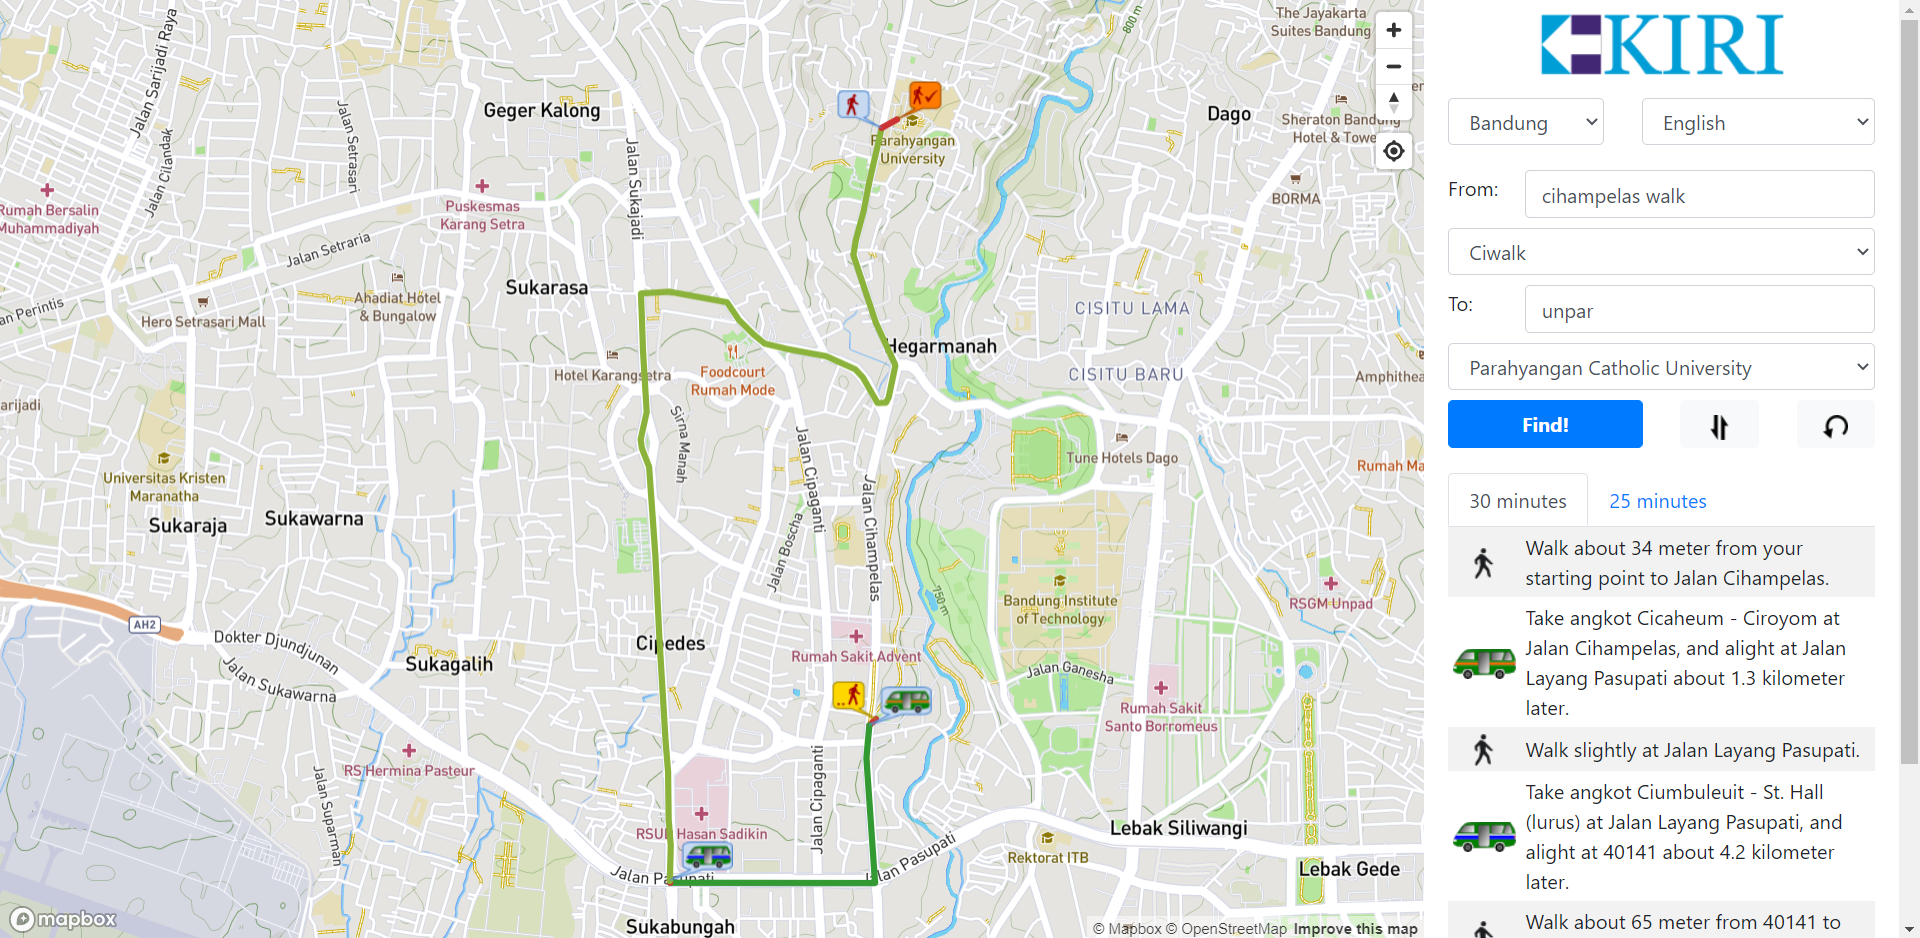
\includegraphics[width=0.74\linewidth]{projectkiri}
    \caption[Tampilan halaman web KIRI]{Tampilan halaman web KIRI, yang menunjukkan rute dari Cihampelas Walk ke Universitas Katolik Parahyangan.}
    \label{fig:kiripage}
\end{figure}

Sementara itu, dalam komputer, salah satu dari sekian banyak tipe perangkat lunak adalah \textit{command line}. \textit{\mbox{Command} line} adalah perangkat lunak paling sederhana, yang sudah ada sejak pertama kali komputer \mbox{diciptakan}. Perangkat lunak selalu memiliki tampilan berupa \cli (CLI), yang \mbox{tidak} \mbox{memiliki} tampilan apapun selain sebuah kotak yang memuat teks berupa perintah-perintah tertentu, \mbox{baik} perintah yang meminta masukan dari user untuk dilakukan oleh komputer, maupun perintah yang menampilkan keluaran dari komputer, tanpa ada tambahan gambar grafis apapun, seperti pada perangkat lunak dengan tampilan \textit{graphical user interface} (GUI). Singkatnya, tipe perangkat lunak ini bukan merupakan tipe yang paling indah untuk dilihat oleh para pengguna, tetapi jika digunakan dengan tepat, maka \mbox{jenis} \mbox{perangkat} lunak ini bisa menyuruh komputer untuk melakukan banyak sekali perintah-perintah dengan sangat cepat dan sangat efektif.

Pada skripsi ini akan dibuat sebuah perangkat lunak berupa perkakas \cl (\textit{command line tool}) yang dapat menjalankan fungsi-fungsi API dari KIRI. Perangkat lunak ini, seperti jenisnya, akan dibuat murni sebagai perkakas yang dijalankan dari \cl (terminal, cmd, PowerShell, dll.), dan tampilan akhir dari perangkat lunak akan berupa \cli tanpa tambahan \textit{graphical user interface}. Keseluruhan dari perangkat lunak ini akan dibangun dalam bahasa C.

\section{Rumusan Masalah}
\begin{enumerate}
	\item Bagaimana membangun perkakas \textit{command line} yang dapat mengimplementasikan fitur-fitur API KIRI dalam bahasa C?
	\item Bagaimana integrasi perkakas \textit{command line} KIRI dapat dilakukan dengan perkakas-perkakas \textit{command line} lainnya di Linux?
\end{enumerate}

\section{Tujuan}
\begin{enumerate}
	\item Membangun perkakas \textit{command line} yang dapat mengimplementasikan fitur-fitur API KIRI dalam bahasa C.
	\item Melakukan integrasi perkakas \textit{command line} KIRI dengan perkakas-perkakas \textit{command line} lainnya di Linux.
\end{enumerate}

\section{Deskripsi Perangkat Lunak}
Perangkat lunak akhir yang akan dibuat memiliki fitur minimal sebagai berikut:
\begin{itemize}
	\item Pengguna dapat memasukkan lokasi awal dan tujuan akhir sebagai masukan dari perangkat lunak.
	\item Pengguna dapat melihat langkah-langkah yang harus ditempuh dalam perjalanan, mulai dari angkot mana saja yang harus dinaiki, ke mana pengguna harus berjalan kaki untuk bisa mencapai angkot terdekat dari lokasi terakhir pengguna, sampai seberapa jauh pengguna harus berjalan untuk mencapai tujuan akhir.
	\item Pengguna dapat melihat jarak yang harus ditempuh untuk setiap langkahnya.
	\item Pengguna dapat melihat seberapa lama waktu perjalanan untuk setiap langkahnya.
\end{itemize}

\section{Detail Pengerjaan Skripsi}
Bagian-bagian pekerjaan skripsi ini adalah sebagai berikut :
	\begin{enumerate}
		\item Melakukan eksplorasi fungsi-fungsi perangkat lunak KIRI serta eksplorasi cara implementasi API KIRI.
		\item Mempelajari bahasa pemrograman C serta mempelajari dokumentasi-dokumentasi dari seluruh modul yang dibutuhkan untuk pembuatan perangkat lunak.
		\item Melakukan analisis dan desain perangkat lunak yang akan dibangun.
	    \item Melakukan eksplorasi terhadap \textit{library-library} yang dapat digunakan serta memenuhi spesifikasi dalam pembuatan perangkat lunak.
		\item Melakukan analisis kebutuhan fitur-fitur perangkat lunak dan melakukan eksplorasi \textit{library} yang dapat digunakan dan memenuhi spesifikasi dalam pembuatan perangkat lunak.
		\item Membangun perangkat lunak berdasarkan rancangan yang sudah dibuat, dengan megimplementasikan seluruh modul dan \textit{library} yang telah ditentukan di tahap sebelumnya dalam bahasa C.
		\item Melakukan pengujian fungsional dan perbaikan \textit{bug}.
		\item Menulis dokumentasi perangkat lunak.
		\item Menulis dokumen skripsi.
	\end{enumerate}

\section{Rencana Kerja}
Rincian capaian yang direncanakan di Skripsi 1 adalah sebagai berikut:
\begin{enumerate}
    \item Melakukan eksplorasi fungsi-fungsi perangkat lunak KIRI serta eksplorasi cara implementasi API KIRI.
	\item Mempelajari bahasa pemrograman C serta mempelajari dokumentasi-dokumentasi dari seluruh modul yang dibutuhkan untuk pembuatan perangkat lunak.
	\item Melakukan analisis dan desain perangkat lunak yang akan dibangun.
	\item Melakukan eksplorasi terhadap \textit{library-library} yang dapat digunakan serta memenuhi spesifikasi dalam pembuatan perangkat lunak.
	\item Menulis dokumen skripsi untuk bagian-bagian yang tidak membutuhkan perangkat lunak yang dibuat untuk selesai terlebih dahulu.
\end{enumerate}

Sedangkan yang akan diselesaikan di Skripsi 2 adalah sebagai berikut:
\begin{enumerate}
    \item Membangun perangkat lunak berdasarkan rancangan yang sudah dibuat, dengan megimplementasikan seluruh modul dan \textit{library} yang telah ditentukan di tahap sebelumnya dalam bahasa C.
	\item Melakukan pengujian fungsional dan perbaikan \textit{bug}.
	\item Menulis dokumentasi perangkat lunak.
	\item Menyelesaikan dokumen skripsi.
\end{enumerate}

\vspace{0.325cm}
\centering Bandung, \tanggal\\
\vspace{2cm} \nama \\ 
\vspace{0.5cm}

Menyetujui, \\
\ifdefstring{\jumpemb}{2}{
\vspace{1.5cm}
\begin{centering} Menyetujui,\\ \end{centering} \vspace{0.75cm}
\begin{minipage}[b]{0.45\linewidth}
% \centering Bandung, \makebox[0.5cm]{\hrulefill}/\makebox[0.5cm]{\hrulefill}/2013 \\
\vspace{2cm} Nama: \makebox[3cm]{\hrulefill}\\ Pembimbing Utama
\end{minipage} \hspace{0.5cm}
\begin{minipage}[b]{0.45\linewidth}
% \centering Bandung, \makebox[0.5cm]{\hrulefill}/\makebox[0.5cm]{\hrulefill}/2013\\
\vspace{2cm} Nama: \makebox[3cm]{\hrulefill}\\ Pembimbing Pendamping
\end{minipage}
\vspace{0.5cm}
}{
% \centering Bandung, \makebox[0.5cm]{\hrulefill}/\makebox[0.5cm]{\hrulefill}/2013\\
\vspace{2cm} \namapemb\\ Pembimbing Tunggal
}

\end{document}